\section{12 Sep 23 - Activity: The Dynamical Systems Approach and Phase
Portraits}\label{sep-23---activity-the-dynamical-systems-approach-and-phase-portraits}

Up to now, most of your work with models in physics are those you can
solve analytically in terms of known functions. Think about solving
differential equations that produce polynomials or sines and cosines.

But what happens when the solution to the problem is not obviously
tractable in an analytical form. Rather, how can we investigate systems
that are new to us?

In today's activity you will:

\begin{itemize}
\tightlist
\item
  Remind yourself how to interpret a 1d phase portrait using the
  differential equation \(\dot{x} = x^2 + 1\)
\item
  Remind yourself how to interpret a 2d phase portrait (phase space
  plot) using the SHO model
\item
  Explain what you see in the phase space figure for the SHO
\item
  Develop the ODE for the large angle pendulum
\item
  Show how we can recover the SHO using mathematics and graphs
\item
  Use an existing program to work with a new system
\item
  Explain the insights developed from a phase space plot of the Large
  Angle Pendulum
\end{itemize}

\subsection{1D System}\label{d-system}

Let's look at a simple 1d system first, given by the differential
equation:

\[
\dot{x} = x^2 - 1
\]

Let's start by looking at what the plot of this differential equation
looks like:

\begin{Shaded}
\begin{Highlighting}[]
\ImportTok{import}\NormalTok{ numpy }\ImportTok{as}\NormalTok{ np}
\ImportTok{import}\NormalTok{ matplotlib.pyplot }\ImportTok{as}\NormalTok{ plt}
\NormalTok{x }\OperatorTok{=}\NormalTok{ np.arange(}\OperatorTok{{-}}\DecValTok{2}\NormalTok{,}\DecValTok{2}\NormalTok{,}\FloatTok{0.01}\NormalTok{)}
\NormalTok{xdot }\OperatorTok{=}\NormalTok{ x}\OperatorTok{**}\DecValTok{2} \OperatorTok{{-}} \DecValTok{1}
\NormalTok{plt.title(}\VerbatimStringTok{r"}\DecValTok{$\textbackslash{}d}\VerbatimStringTok{ot\{x\} = x}\DecValTok{\^{}}\VerbatimStringTok{2 {-} 1}\DecValTok{$}\VerbatimStringTok{"}\NormalTok{)}
\NormalTok{plt.axvline(x}\OperatorTok{=}\DecValTok{0}\NormalTok{, c}\OperatorTok{=}\StringTok{"black"}\NormalTok{)}
\NormalTok{plt.axhline(y}\OperatorTok{=}\DecValTok{0}\NormalTok{, c}\OperatorTok{=}\StringTok{"black"}\NormalTok{)}
\NormalTok{plt.plot(x,xdot)}
\NormalTok{plt.grid()}
\NormalTok{plt.show()}
\end{Highlighting}
\end{Shaded}

\begin{figure}
\centering
\pandocbounded{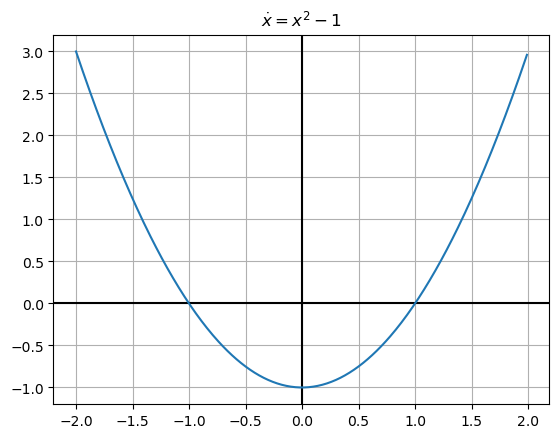
\includegraphics[keepaspectratio,alt={png}]{../images/activity-phase_space_activity-phase_space_tmp_2_0.png}}
\caption{png}
\end{figure}

Since this is a first order equation we have a nice physical way of
thinking about it: at position \(x\), a particles velocity is
\(x^2 -1\). So when the \(x^2-1\) is positive, the particle's velocity
is positive (or to the right) and vice versa. We can use this knowledge
to work out qualitative behavor of our system.

\textbf{✅ Do this}

\begin{enumerate}
\def\labelenumi{\arabic{enumi}.}
\tightlist
\item
  Consider a trajectory that starts at \(x = -1.5\). Does this
  trajectory move to the right or left?
\item
  What direction does a trajectory that starts at \(x = 0\) go?
\item
  What direction does a trajectory that starts at \$ x = 1.5\$ go?
\item
  What trends do you notice? Do trajectories settle down at certain
  locations or blast off to infinity?
\end{enumerate}

\subsubsection{Fixed Points}\label{fixed-points}

The \textbf{fixed points} of a system are where its derivative vanishes,
that is \(\dot{\mathbf{x}} = 0\). At any fixed point, a system is
constant (why?). In the dynamical systems approach, we often care about
charactarizing the behavor of systems near fixed points. In 1d, most
fixed points are either stable (they attract trajectories) or unstable
(they repel trajectories).

\textbf{✅ Do this}

Find and characterize the fixed points of \(\dot{x} = x^2-1\) as stable
or unstable.

Another way we can visualize these is with \textbf{slope fields}. Here
we essentially plot the slopes \(\dot{x}(x)\) over and over again for
many values of \(t\). The actual solution of the differential equation
will be a curve that is always tangent to the local slope. Below we've
plotted this using both \texttt{plt.quiver} and \texttt{plt.streamplot}

\begin{Shaded}
\begin{Highlighting}[]
\ImportTok{import}\NormalTok{ numpy }\ImportTok{as}\NormalTok{ np}
\ImportTok{import}\NormalTok{ matplotlib.pyplot }\ImportTok{as}\NormalTok{ plt}

\NormalTok{t }\OperatorTok{=}\NormalTok{ np.arange(}\DecValTok{0}\NormalTok{, }\DecValTok{11}\NormalTok{, }\FloatTok{0.8}\NormalTok{)}
\NormalTok{x }\OperatorTok{=}\NormalTok{ np.arange(}\OperatorTok{{-}}\DecValTok{2}\NormalTok{, }\DecValTok{2}\NormalTok{, }\FloatTok{0.4}\NormalTok{)}

\CommentTok{\# Make grid}
\NormalTok{T, X }\OperatorTok{=}\NormalTok{ np.meshgrid(t, x)}

\CommentTok{\# calculate derivative (dt is const so just use ones)}
\NormalTok{dx }\OperatorTok{=}\NormalTok{ X}\OperatorTok{**}\DecValTok{2} \OperatorTok{{-}} \DecValTok{1}
\NormalTok{dt }\OperatorTok{=}\NormalTok{ np.ones(dx.shape)}

\CommentTok{\# plot}
\NormalTok{fig }\OperatorTok{=}\NormalTok{ plt.figure(figsize }\OperatorTok{=}\NormalTok{ (}\DecValTok{10}\NormalTok{,}\DecValTok{5}\NormalTok{))}
\NormalTok{plt.subplot(}\DecValTok{1}\NormalTok{,}\DecValTok{2}\NormalTok{,}\DecValTok{1}\NormalTok{)}
\NormalTok{plt.quiver(T,X,dt,dx)}
\NormalTok{plt.xlabel(}\StringTok{"t"}\NormalTok{)}
\NormalTok{plt.ylabel(}\StringTok{"x"}\NormalTok{)}
\NormalTok{plt.subplot(}\DecValTok{1}\NormalTok{,}\DecValTok{2}\NormalTok{,}\DecValTok{2}\NormalTok{)}
\NormalTok{plt.streamplot(T,X,dt,dx)}
\NormalTok{plt.xlabel(}\StringTok{"t"}\NormalTok{)}
\NormalTok{plt.ylabel(}\StringTok{"x"}\NormalTok{)}
\NormalTok{plt.suptitle(}\StringTok{"Slope Field"}\NormalTok{)}
\NormalTok{plt.show()}
\end{Highlighting}
\end{Shaded}

\begin{figure}
\centering
\pandocbounded{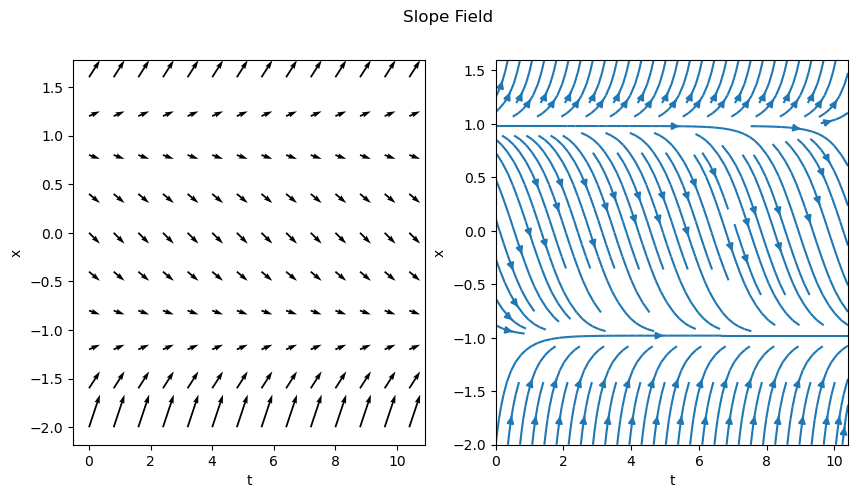
\includegraphics[keepaspectratio,alt={png}]{../images/activity-phase_space_activity-phase_space_tmp_5_0.png}}
\caption{png}
\end{figure}

\subsection{Reminders about the SHO}\label{reminders-about-the-sho}

To get this started, let's remind ourselves of the phase portrait of the
SHO. Recall that we separated the second order ODE into two first order
ODEs, one for \(x\) and one for \(v_x\),

\[\dot{x} = v_x\] \[\dot{v}_x=-\omega^2x\]

We then map out the phase space with the following conceptual
interpretation:

\begin{itemize}
\tightlist
\item
  Phase space is a space in which all possible states of the system can
  be shown

  \begin{itemize}
  \tightlist
  \item
    a state is a collection of conditions of the state (it's known
    position and velocity in our case)
  \end{itemize}
\item
  Each state is a unique point in phase space

  \begin{itemize}
  \tightlist
  \item
    Think about ordered Cartesian pairs, there's a pair of numbers for
    every point in a 2D space
  \end{itemize}
\item
  Remember that knowing \(x_0\) and \(v_{x,0}\) means we can know
  \(x(t)\) for all time (for that one trajectory/particular solution)
  given a linear ODE
\end{itemize}

We map the differential equation to the following conceptual
interpretation: \textbf{How the state changes depends on location in
phase space.} We can understand this as the time derivative for \(x\)
and \(v_x\) change throughout the space.

For our 2D SHO case we are saying that how \(x\) and \(v_x\) change is
proportional to the position in space:

\[\langle \dot{x}, \dot{v}_x \rangle = \langle v_x, -\omega^2 x\rangle\]

The process is:

\begin{enumerate}
\def\labelenumi{\arabic{enumi}.}
\tightlist
\item
  Determine the location(s) of interest (i.e., \(x\), \(v_x\))
\item
  Compute the change in those quantities at the location (i.e.,
  calculate \(\dot{x}\) and \(\dot{v}_x\) using our prescribed 1st order
  ODEs above)
\item
  At a given point (\(x_0\), \(v_{x,0}\)), create an arrow the indicates
  the direction and magnitude of the changes to \(x\) and \(v_x\) at
  that location.

  \begin{itemize}
  \tightlist
  \item
    That arrow represents the local flow of the system at that point
  \end{itemize}
\item
  Repeat for all points of interest
\item
  Plot arrows to demonstrate flow of the solutions in phase space
\end{enumerate}

\subsection{Phase Portrait of the Simple Harmonic
Oscillator}\label{phase-portrait-of-the-simple-harmonic-oscillator}

Below, we have written code that makes a phase portrait from the simple
harmonic oscillator. It's written in terms of three functions that serve
three purposes that you might want to modify in your own work:

\begin{itemize}
\tightlist
\item
  \texttt{SHOPhasePortrait} is a function that simply returns the
  relationship between the locations in phase space and how the phase
  variables change at that location.
\item
  \texttt{ComputeSHOPhase} is a function that uses that relationship and
  computes the values of the changes at every location. It returns two
  arrays, which contain all those values.
\item
  \texttt{SHOTrajectory} is a function that takes a pair of points in
  space and computes the trajectory in phase space
\end{itemize}

By separating these ideas, we are illustrating the process for computing
these phase portraits: - Translate one \(Nth\) order differential
equation to \(N\) 1st order (Done earlier in this case) - Put that into
a code so you can compute the value of the changes at a location
(\texttt{SHOPhasePotrait}) - Call that computation a bunch to compute it
at every location you want (\texttt{ComputeSHOPhase}) - investigate
specific trajectories in the space (\texttt{SHOTrajectory})

We can then call these functions can plots the results.

\begin{Shaded}
\begin{Highlighting}[]
\KeywordTok{def}\NormalTok{ SHOPhasePortrait(x, vx, omega):}
    \CommentTok{\textquotesingle{}\textquotesingle{}\textquotesingle{}SHOPhasePortrait returns the value of}
\CommentTok{    the change in the phase variables at a given location}
\CommentTok{    in phase space for the SHO model\textquotesingle{}\textquotesingle{}\textquotesingle{}}
    
\NormalTok{    xdot, vxdot }\OperatorTok{=}\NormalTok{ [vx, }\OperatorTok{{-}}\DecValTok{1}\OperatorTok{*}\NormalTok{omega}\OperatorTok{**}\DecValTok{2}\OperatorTok{*}\NormalTok{x] }\CommentTok{\#\# Specific to this problem}
    
    \ControlFlowTok{return}\NormalTok{ xdot, vxdot}

\KeywordTok{def}\NormalTok{ ComputeSHOPhase(X, VX, omega):}
    \CommentTok{\textquotesingle{}\textquotesingle{}\textquotesingle{}ComputeSHOPhase returns the changes in }
\CommentTok{    the phase variables across a grid of locations}
\CommentTok{    that are specified\textquotesingle{}\textquotesingle{}\textquotesingle{}}
    
    \CommentTok{\#\# Prep the arrays with zeros at the right size}
\NormalTok{    xdot, vxdot }\OperatorTok{=}\NormalTok{ np.zeros(X.shape), np.zeros(VX.shape)}

    \CommentTok{\#\# Set the limits of the loop based on how }
    \CommentTok{\#\# many points in the arrays we have}
\NormalTok{    Xlim, Ylim }\OperatorTok{=}\NormalTok{ X.shape}
    
    \CommentTok{\#\# Calculate the changes at each location and add them to the arrays}
    \ControlFlowTok{for}\NormalTok{ i }\KeywordTok{in} \BuiltInTok{range}\NormalTok{(Xlim):}
        \ControlFlowTok{for}\NormalTok{ j }\KeywordTok{in} \BuiltInTok{range}\NormalTok{(Ylim):}
\NormalTok{            xloc }\OperatorTok{=}\NormalTok{ X[i, j]}
\NormalTok{            yloc }\OperatorTok{=}\NormalTok{ VX[i, j]}
\NormalTok{            xdot[i,j], vxdot[i,j] }\OperatorTok{=}\NormalTok{ SHOPhasePortrait(xloc, yloc, omega)}
            
    \ControlFlowTok{return}\NormalTok{ xdot, vxdot}

\KeywordTok{def}\NormalTok{ SHOTrajectory(x0, vx0, omega, N}\OperatorTok{=}\DecValTok{100}\NormalTok{):}
    \CommentTok{\textquotesingle{}\textquotesingle{}\textquotesingle{}SHOTrajectory computes the phase space}
\CommentTok{    trjectory using the analytical forms of the}
\CommentTok{    solution. Note this sloppy analytical approach}
\CommentTok{    only works because the SHO is perfectly sinusoidal.\textquotesingle{}\textquotesingle{}\textquotesingle{}}
    
    \CommentTok{\#\# Only work with one period}
\NormalTok{    T }\OperatorTok{=} \DecValTok{2}\OperatorTok{*}\NormalTok{np.pi}\OperatorTok{/}\NormalTok{omega}
\NormalTok{    t }\OperatorTok{=}\NormalTok{ np.arange(}\DecValTok{0}\NormalTok{,T,T}\OperatorTok{/}\NormalTok{N)}
    
    \CommentTok{\#\# I derived this in general with Acos(wt+phi)}
    \CommentTok{\#\# It\textquotesingle{}s not in general a good approach}
    \CommentTok{\#\# because you are not guaranteed analytical }
    \CommentTok{\#\# closed form trajectories in phase space}
    
\NormalTok{    phi }\OperatorTok{=}\NormalTok{ np.arctan2(}\OperatorTok{{-}}\DecValTok{1}\OperatorTok{*}\NormalTok{vx0, omega}\OperatorTok{*}\NormalTok{x0) }\CommentTok{\#\# arctan({-}vxo/(omega*x0)) taken correctly for the quadrant}
\NormalTok{    A }\OperatorTok{=}\NormalTok{ x0}\OperatorTok{/}\NormalTok{np.cos(phi)}
\NormalTok{    x\_traj }\OperatorTok{=}\NormalTok{ A}\OperatorTok{*}\NormalTok{np.cos(omega}\OperatorTok{*}\NormalTok{t}\OperatorTok{+}\NormalTok{phi)}
\NormalTok{    v\_traj }\OperatorTok{=} \OperatorTok{{-}}\NormalTok{omega}\OperatorTok{*}\NormalTok{A}\OperatorTok{*}\NormalTok{np.sin(omega}\OperatorTok{*}\NormalTok{t}\OperatorTok{+}\NormalTok{phi)}
    
    \ControlFlowTok{return}\NormalTok{ x\_traj, v\_traj}
\end{Highlighting}
\end{Shaded}

\subsubsection{Putting the functions to
use}\label{putting-the-functions-to-use}

With these two functions, all we are left to do is specify the size of
the space and the grid points (that is where exactly we are computing
the changes). We use
\href{https://numpy.org/doc/stable/reference/generated/numpy.meshgrid.html}{meshgrid}
to make those arrays a set of Cartesian coordinates and then send that
to our functions.

We then plot the results.

\begin{Shaded}
\begin{Highlighting}[]
\CommentTok{\#\# Setting parameters and the phase space variables}

\NormalTok{omega }\OperatorTok{=} \DecValTok{1}
\NormalTok{x }\OperatorTok{=}\NormalTok{ np.linspace(}\OperatorTok{{-}}\FloatTok{10.0}\NormalTok{, }\FloatTok{10.0}\NormalTok{, }\DecValTok{20}\NormalTok{)}
\NormalTok{vx }\OperatorTok{=}\NormalTok{ np.linspace(}\OperatorTok{{-}}\FloatTok{10.0}\NormalTok{, }\FloatTok{10.0}\NormalTok{, }\DecValTok{20}\NormalTok{)}

\CommentTok{\#\# Get back pairs of coordinates for every point in the space}
\NormalTok{X, VX }\OperatorTok{=}\NormalTok{ np.meshgrid(x, vx)}

\CommentTok{\#\# Run our calculations}
\NormalTok{xdot, vxdot }\OperatorTok{=}\NormalTok{ ComputeSHOPhase(X, VX, omega)}

\NormalTok{x0 }\OperatorTok{=} \DecValTok{5}
\NormalTok{vx0 }\OperatorTok{=} \DecValTok{3}
\NormalTok{x\_traj, v\_traj }\OperatorTok{=}\NormalTok{ SHOTrajectory(x0, vx0, omega)}

\CommentTok{\#\# Plot. plot. plot.}
\NormalTok{ax }\OperatorTok{=}\NormalTok{ plt.figure(figsize}\OperatorTok{=}\NormalTok{(}\DecValTok{15}\NormalTok{,}\DecValTok{7}\NormalTok{))}
\NormalTok{plt.subplot(}\DecValTok{1}\NormalTok{,}\DecValTok{2}\NormalTok{,}\DecValTok{1}\NormalTok{)}

\CommentTok{\#\# Plot with Quiver}
\NormalTok{Q }\OperatorTok{=}\NormalTok{ plt.quiver(X, VX, xdot, vxdot, color}\OperatorTok{=}\StringTok{\textquotesingle{}k\textquotesingle{}}\NormalTok{)}

\CommentTok{\#\# Plot trajectory and the starting location}
\NormalTok{plt.plot(x\_traj,v\_traj)}
\NormalTok{plt.plot(x0, vx0, }\StringTok{\textquotesingle{}r*\textquotesingle{}}\NormalTok{, markersize}\OperatorTok{=}\DecValTok{10}\NormalTok{)}

\NormalTok{plt.xlabel(}\StringTok{\textquotesingle{}$x$\textquotesingle{}}\NormalTok{)}
\NormalTok{plt.ylabel(}\StringTok{\textquotesingle{}$v\_x$\textquotesingle{}}\NormalTok{)}
\NormalTok{plt.grid()}

\NormalTok{plt.subplot(}\DecValTok{1}\NormalTok{,}\DecValTok{2}\NormalTok{,}\DecValTok{2}\NormalTok{)}
\CommentTok{\#\# Plot with streamplot for subplot}
\NormalTok{Q }\OperatorTok{=}\NormalTok{ plt.streamplot(X, VX, xdot, vxdot, color}\OperatorTok{=}\StringTok{\textquotesingle{}k\textquotesingle{}}\NormalTok{)}
\NormalTok{plt.plot(x\_traj,v\_traj)}
\NormalTok{plt.plot(x0, vx0, }\StringTok{\textquotesingle{}r*\textquotesingle{}}\NormalTok{, markersize}\OperatorTok{=}\DecValTok{10}\NormalTok{)}

\NormalTok{plt.xlabel(}\StringTok{\textquotesingle{}$x$\textquotesingle{}}\NormalTok{)}
\NormalTok{plt.ylabel(}\StringTok{\textquotesingle{}$v\_x$\textquotesingle{}}\NormalTok{)}
\NormalTok{plt.grid()}
\end{Highlighting}
\end{Shaded}

\begin{figure}
\centering
\pandocbounded{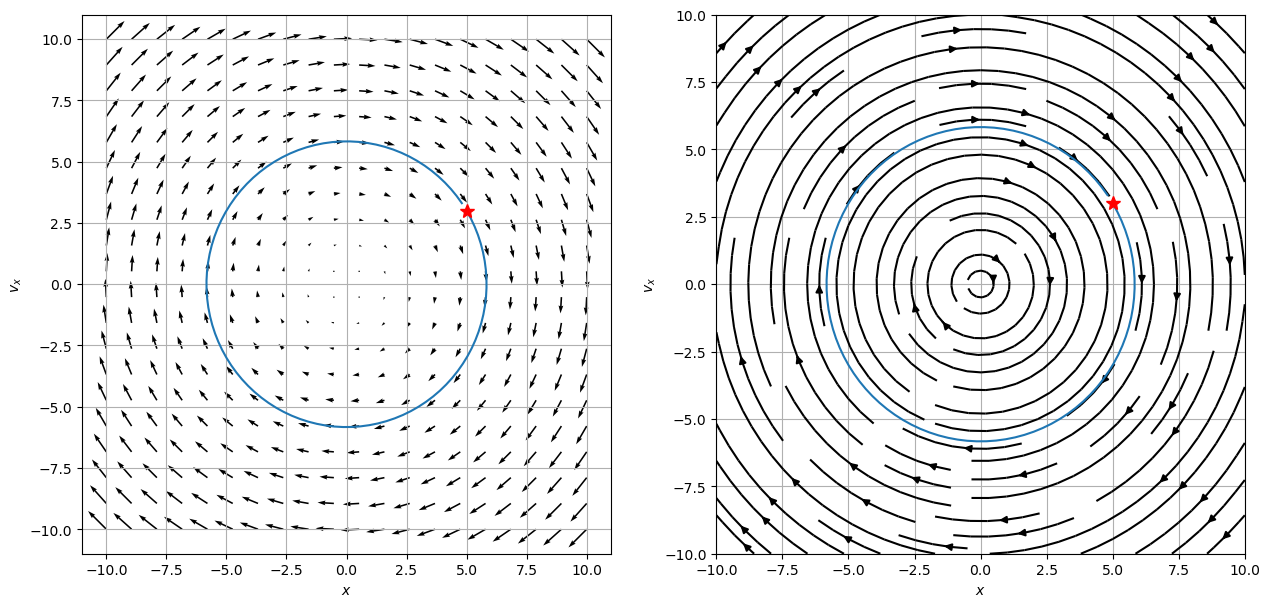
\includegraphics[keepaspectratio,alt={png}]{../images/activity-phase_space_activity-phase_space_tmp_10_0.png}}
\caption{png}
\end{figure}

\subsubsection{What can phase space help us
do?}\label{what-can-phase-space-help-us-do}

\textbf{✅ Do this}

Let's remember a few things about the SHO.

\begin{enumerate}
\def\labelenumi{\arabic{enumi}.}
\tightlist
\item
  With your neighbors, list all the things you know about the SHO.
  Include anything we haven't discussed (e.g., the energetics of the
  problem).
\item
  Name which of those things you can see in the phase diagram. Which
  things are you sure you can see? What things don't seem to be able to
  be seen from the phase diagram?
\item
  What do you remember about the energy of an SHO? Consider a harmonic
  oscillator in a known trajectory (\(x(t) = A\cos(\omega t)\)). Compute
  the total (conserved) energy of the oscillator as a function of time.

  \begin{itemize}
  \tightlist
  \item
    Explain how your expression for energy conservation can be seen in
    your phase diagram.
  \item
    You might try to show analytically that the ellipse above is related
    to your energy conservation expression
  \end{itemize}
\item
  What are the fixed points for this system? Can it be classified as
  stable/unstable or do we need to think of something new?
\end{enumerate}

What do these plots tell you about all potential solutions?

\subsection{The Large Angle Pendulum}\label{the-large-angle-pendulum}

The Large Angle Pendulum is the first of a number of nonlinear
differential equations out there. This one is quite special in that the
integral that solves for the period of this pendulum has a name! It's
called and
\href{https://en.wikipedia.org/wiki/Elliptic_integral}{Elliptical
Integral of the First Kind}. Elliptical because of the nature of the
kernel of the integral, which has an elliptic form (in our case, one
over the square root of a quantity squared subtracted from one, yes,
seriously, we have a name for that).

Here's the pendulum in all it's glory.

\begin{figure}
\centering
\pandocbounded{\includegraphics[keepaspectratio,alt={Large Angle Pendulum}]{../images/activity-phase_space_pendulum_bob.png}}
\caption{Large Angle Pendulum}
\end{figure}

The analytical solution for the period is given by:

\[T = 4\sqrt{\dfrac{L}{g}}\int_0^{\pi/2}\dfrac{d\theta}{\sqrt{1-k^2\sin^2(\theta)}}\]

To find the period, we have to use some form of computation, even it's
the ``well-known''
\href{https://en.wikipedia.org/wiki/Elliptic_integral\#Complete_elliptic_integral_of_the_first_kind}{recurrence
relationship} that was used for centuries to compute this integral
\textbf{by hand}.

But let's try to gain insight from the phase space instead. We can
{[}derive{]} the differential equation that describes the motion of the
pendulum through an angle \(\theta\) thusly:

\[\ddot{\theta} = -\dfrac{g}{L}\sin(\theta)\]

You have a second order differential equation for \(\theta\).

\subsubsection{Make a new phase
portrait}\label{make-a-new-phase-portrait}

\textbf{✅ Do this}

With your partners,

\begin{enumerate}
\def\labelenumi{\arabic{enumi}.}
\tightlist
\item
  Take the 2nd order ODE and make it two 1st order ODEs (one for
  \(\theta\) and one for \(\omega=\dot{\theta}\)). Make sure you agree
  on the analytics.
\item
  Add those expressions to the function \texttt{LAPPhasePortrait}
\item
  The rest of the code runs the same as before (we've engaged in
  reproducible and adaptable work!), so make some phase portraits.

  \begin{itemize}
  \tightlist
  \item
    What do you notice?
  \item
    What physics is new?
  \item
    What physics is old?
  \end{itemize}
\item
  Play with parameters and build a story for what is going on with the
  motion.
\end{enumerate}

\begin{Shaded}
\begin{Highlighting}[]
\KeywordTok{def}\NormalTok{ LAPPhasePortrait(x, vx, omega0 }\OperatorTok{=} \DecValTok{10}\NormalTok{):}
    
    \CommentTok{\#\#\#\#\#\#\#\#\#\#\#\#\#\#\#\#\#}
    \CommentTok{\#\# CHANGE THIS \#\#}
    \CommentTok{\#\#\#\#\#\#\#\#\#\#\#\#\#\#\#\#\#}
\NormalTok{    xdot, vxdot }\OperatorTok{=}\NormalTok{ [}\DecValTok{1}\NormalTok{, }\DecValTok{1}\NormalTok{] }\CommentTok{\#\# Specific to the problem}
    
    \ControlFlowTok{return}\NormalTok{ xdot, vxdot}

\KeywordTok{def}\NormalTok{ ComputeLAPPhase(X, VX, omega0):}
    
\NormalTok{    xdot, vxdot }\OperatorTok{=}\NormalTok{ np.zeros(X.shape), np.zeros(VX.shape)}

\NormalTok{    Xlim, Ylim }\OperatorTok{=}\NormalTok{ X.shape}
    
    \ControlFlowTok{for}\NormalTok{ i }\KeywordTok{in} \BuiltInTok{range}\NormalTok{(Xlim):}
        \ControlFlowTok{for}\NormalTok{ j }\KeywordTok{in} \BuiltInTok{range}\NormalTok{(Ylim):}
\NormalTok{            xloc }\OperatorTok{=}\NormalTok{ X[i, j]}
\NormalTok{            yloc }\OperatorTok{=}\NormalTok{ VX[i, j]}
\NormalTok{            xdot[i,j], vxdot[i,j] }\OperatorTok{=}\NormalTok{ LAPPhasePortrait(xloc, yloc, omega0)}
            
    \ControlFlowTok{return}\NormalTok{ xdot, vxdot}

\NormalTok{omega0 }\OperatorTok{=} \DecValTok{2}
\NormalTok{N }\OperatorTok{=} \DecValTok{40}

\NormalTok{x }\OperatorTok{=}\NormalTok{ np.linspace(}\OperatorTok{{-}}\FloatTok{6.0}\NormalTok{, }\FloatTok{6.0}\NormalTok{, N)}
\NormalTok{vx }\OperatorTok{=}\NormalTok{ np.linspace(}\OperatorTok{{-}}\FloatTok{8.0}\NormalTok{, }\FloatTok{8.0}\NormalTok{, N)}

\NormalTok{X, VX }\OperatorTok{=}\NormalTok{ np.meshgrid(x, vx)}

\NormalTok{xdot, vxdot }\OperatorTok{=}\NormalTok{ ComputeLAPPhase(X, VX, omega0)}

\NormalTok{ax }\OperatorTok{=}\NormalTok{ plt.figure(figsize}\OperatorTok{=}\NormalTok{(}\DecValTok{10}\NormalTok{,}\DecValTok{6}\NormalTok{))}
\NormalTok{Q }\OperatorTok{=}\NormalTok{ plt.quiver(X, VX, xdot, vxdot, color}\OperatorTok{=}\StringTok{\textquotesingle{}k\textquotesingle{}}\NormalTok{)}
\NormalTok{plt.grid()}

\NormalTok{plt.xlabel(}\StringTok{\textquotesingle{}$x$\textquotesingle{}}\NormalTok{)}
\NormalTok{plt.ylabel(}\StringTok{\textquotesingle{}$v\_x$\textquotesingle{}}\NormalTok{)}
\NormalTok{plt.show()}
\end{Highlighting}
\end{Shaded}

\begin{figure}
\centering
\pandocbounded{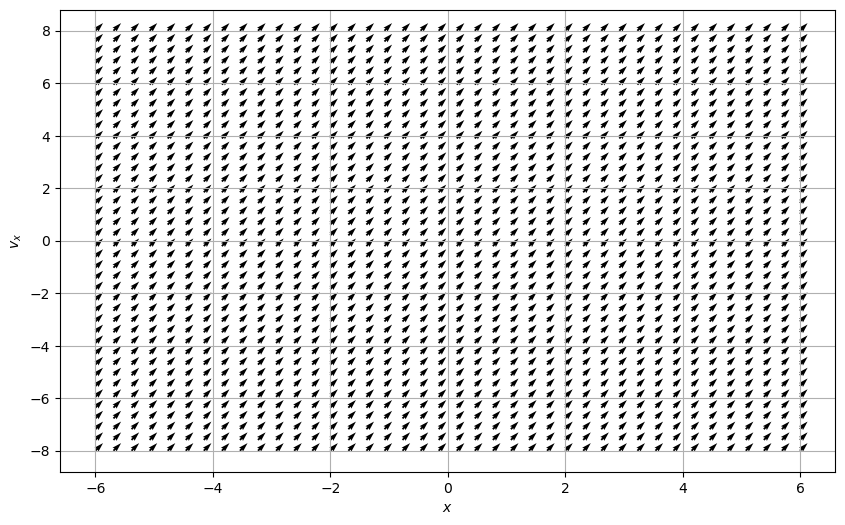
\includegraphics[keepaspectratio,alt={png}]{../images/activity-phase_space_activity-phase_space_tmp_14_0.png}}
\caption{png}
\end{figure}

\textbf{✅ Do this}

Find the fixed points of this system. Are they the same as in the SHO
case? If they're different, what about this system makes it different?

\subsection{(Time Permitting) Fixed Points in 2
Dimensions}\label{time-permitting-fixed-points-in-2-dimensions}

If we don't get to this in class today don't worry, we'll start out with
this on thursday!

Now that we've stepped into two dimensional phase space, the amount of
interesting geometry that our solutions can have is much greater. In
particular, local behavior near fixed points can now exhibit much more
complex behavior than just being stable or not, as we can see in this
figure.

So how do we definitively say what the behavior of our system is like
near a fixed point? The anwer lies in \textbf{linearization}. A linear
system in 2d is a system of the form:

\[
\dot{x} = ax + by \hspace{1in} \dot{y} = cx + dy
\]

Note we can convieniently write this in matrix notation:

\[
\dot{\mathbf{x}} = A\mathbf{x}
\]

Where

\[
A = 
\begin{bmatrix}
a & b \\
c & d
\end{bmatrix}
\hspace{0.5in}\text{and} \hspace{0.5in} \mathbf{x} = \begin{bmatrix} x \\ y \end{bmatrix}
\]

These systems are understood quite well and play very nice
mathematically (see strogatz chapter 5). Miraculously, the mathematical
tools for classifying fixed points of linear systems carry over into
nonlinear systems with little tweaking. This is because most nonlinear
systems behave in linear ways near fixed points. This means we can
\textbf{linearize} nonlinear systems. Here's how you do it:

Suppose you have a system given by:

\[
\dot{x} = f(x,y)
\]

\[
\dot{y} = g(x,y)
\]

With fixed point \((x^*,y^*)\). Near this fixed point, distrubances to
the system will evolve approximatley according to:

\[
\begin{bmatrix} \dot{x} \\ \dot{y} \end{bmatrix} = \begin{bmatrix} \frac{\partial f}{\partial x} & \frac{\partial f}{\partial y} \\ \frac{\partial g}{\partial x} & \frac{\partial g}{\partial y}\end{bmatrix} \begin{bmatrix}x - x^* \\ y - y^*\end{bmatrix}
\]

This is called the \textbf{linearized system}. The matrix

\[
A = \begin{bmatrix} \frac{\partial f}{\partial x} & \frac{\partial f}{\partial y} \\ \frac{\partial g}{\partial x} & \frac{\partial g}{\partial y}\end{bmatrix}_{(x^*,y^*)}
\] is the \textbf{Jacobian matrix} at this fixed point, which is the
multivariable version of the derivative. To categorize the fixed points
of a given system at a fixed point, calculate \(A\) for said fixed
point, then find its Eigenvalues. Recall Eigenvalues are the \(\lambda\)
in \(A\mathbf{v} = \lambda \mathbf{v}\). \(2\times2\) matricies have (up
to) 2 eigenvalues. These eigenvalues tell you about the stability of the
system:

\begin{itemize}
\tightlist
\item
  \$\mathrm{Re}(\lambda) \textgreater{} 0 \$ for both eigenvalues:
  Repeller/Source (unstable)
\item
  \$\mathrm{Re}(\lambda) \textless{} 0 \$ for both eigenvalues:
  Attractor/Sink (stable)
\item
  One eigenvalue positive, one negative: Saddle
\item
  Both eigenvalues pure imaginary: Center
\end{itemize}

In fact one can learn quite a bit more from a these eigenvalues (see
strogatz chapter 6 or section 5.4
\href{https://users.math.msu.edu/users/gnagy/teaching/ode.pdf}{here}),
but these charactarizations are a great starting point.

\begin{Shaded}
\begin{Highlighting}[]

\end{Highlighting}
\end{Shaded}

\textbf{✅ Do this}

Calculate the Jacobian matrix \(A\) for a fixed point of the large angle
pendulum.
